\begin{section}{SG}{Stacking the Cosmic Web in Fluorescent Lyman alpha Emission}
  \begin{minipage}[l]{\textwidth}

    {\small Most of the matter in the Universe seems to be distributed along
      filaments connecting galaxies. Fluorescently illuminated by the light of
      first stars and quasars, their expected surface brightness (SB) in
      Lyalpha is beyond current observational limits. By using the deepest
      MUSE/VLT data available, we perform a stacking analysis around Lyalpha
      emitting galaxies (LAEs) between 3<z<4, with orientations determined by
      neighbouring galaxies, reaching a SB sensitivity level bellow the
      predicted signal. No detectable emission is found on intergalactic
      scales implying most of our selected regions do not contain filaments
      given our adopted model. On the other hand, significant emission is
      found on the circum-galactic medium in the direction of the neighbours,
      suggesting typically larger gas densities on those directions. The
      signal is increased around galaxies with a larger number of neighbours
      but seems independent of any other galaxy properties such as redshift,
      neighbour distance and luminosity.}
  \end{minipage}

  \vspace{0.5cm}

  \begin{minipage}{\linewidth}
    \begin{center}
      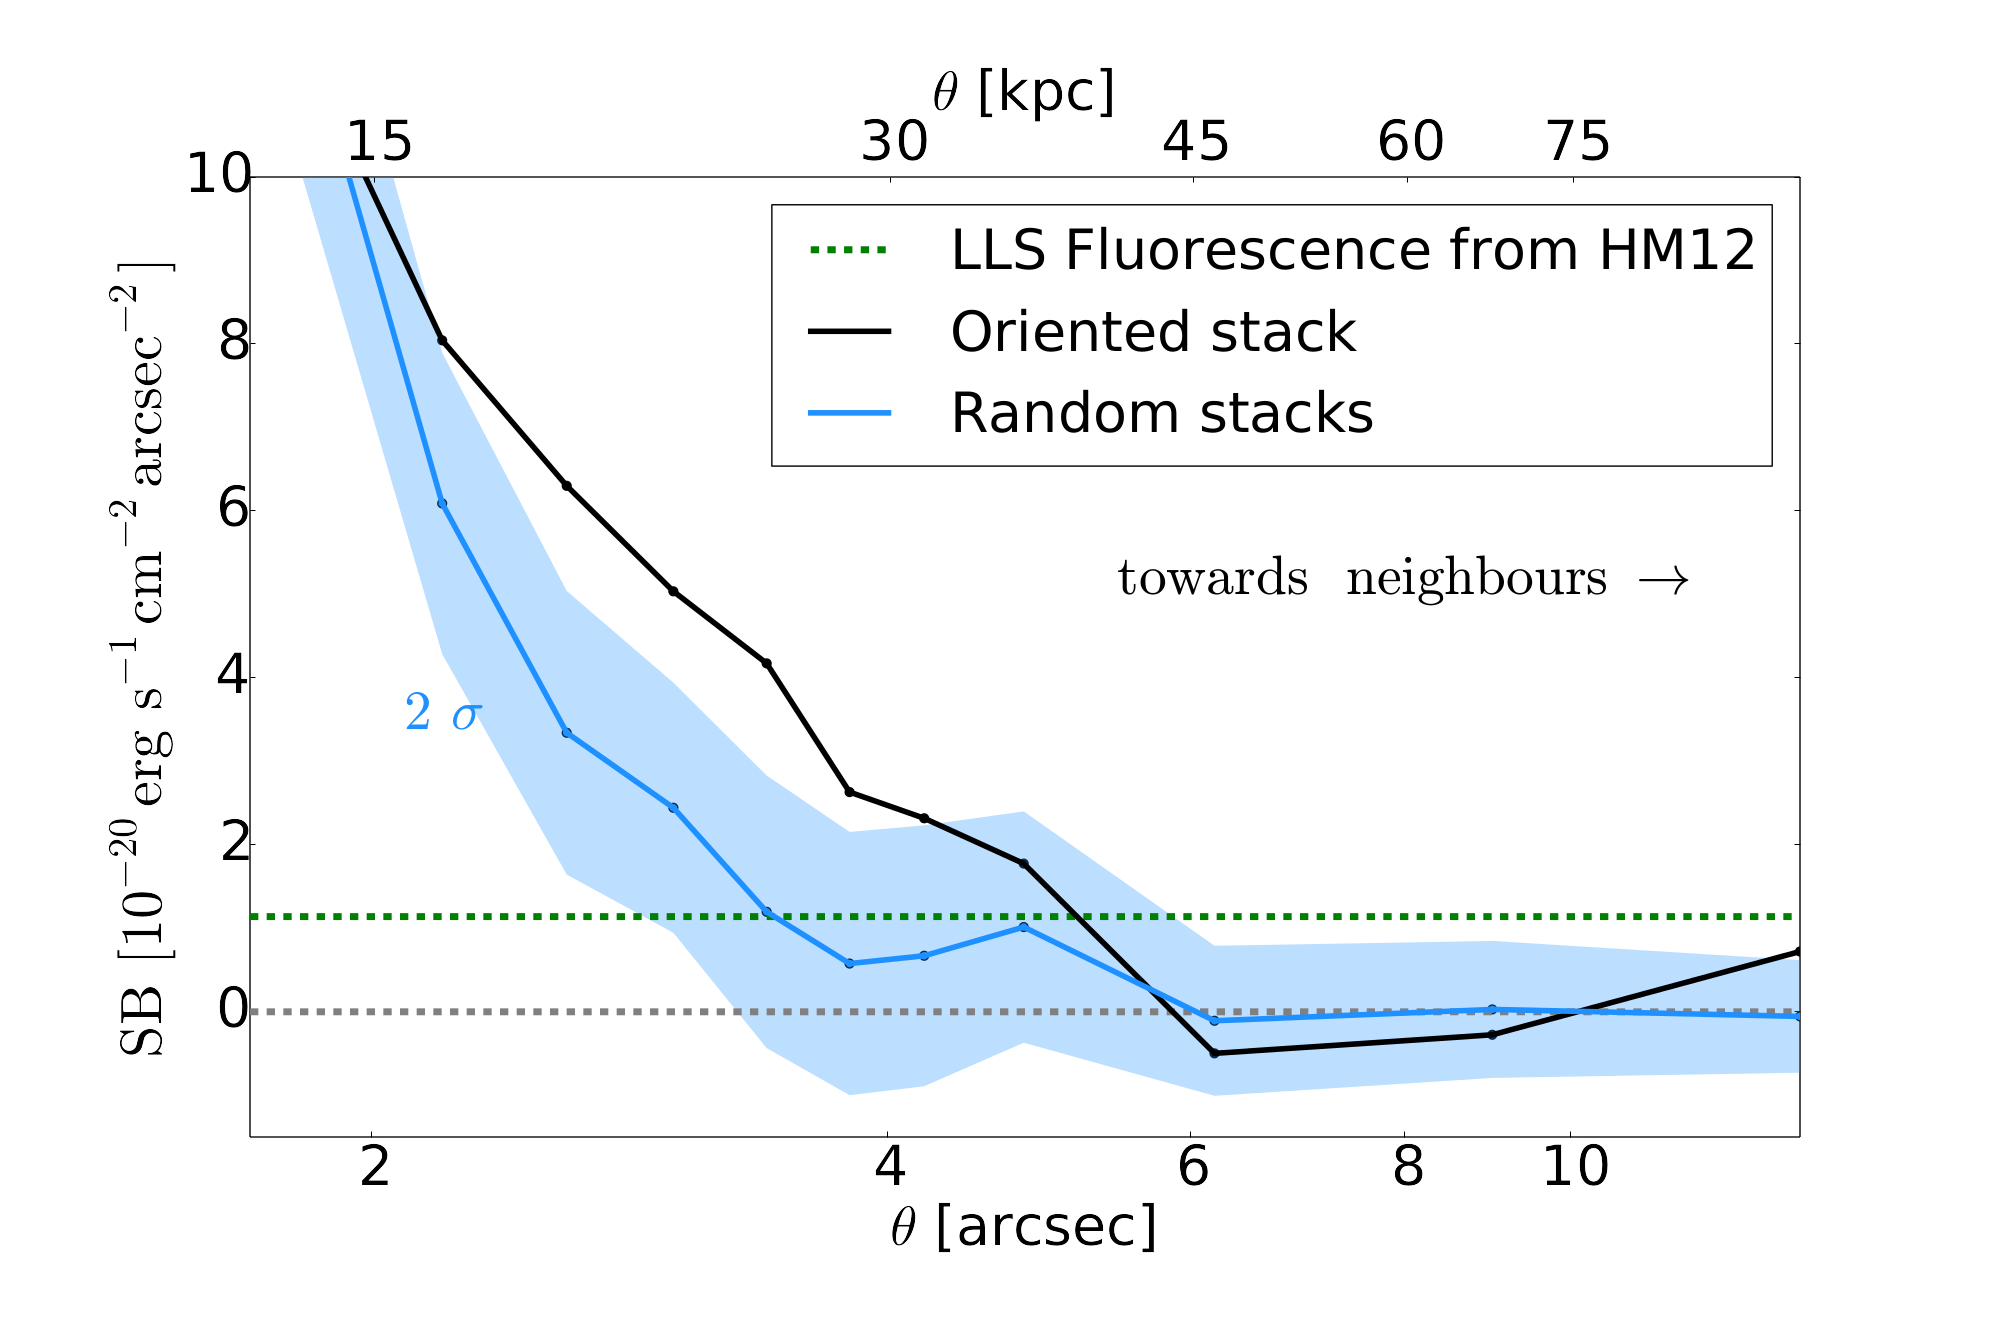
\includegraphics[height=10cm]{SG/SB_right_nmin8.png}
      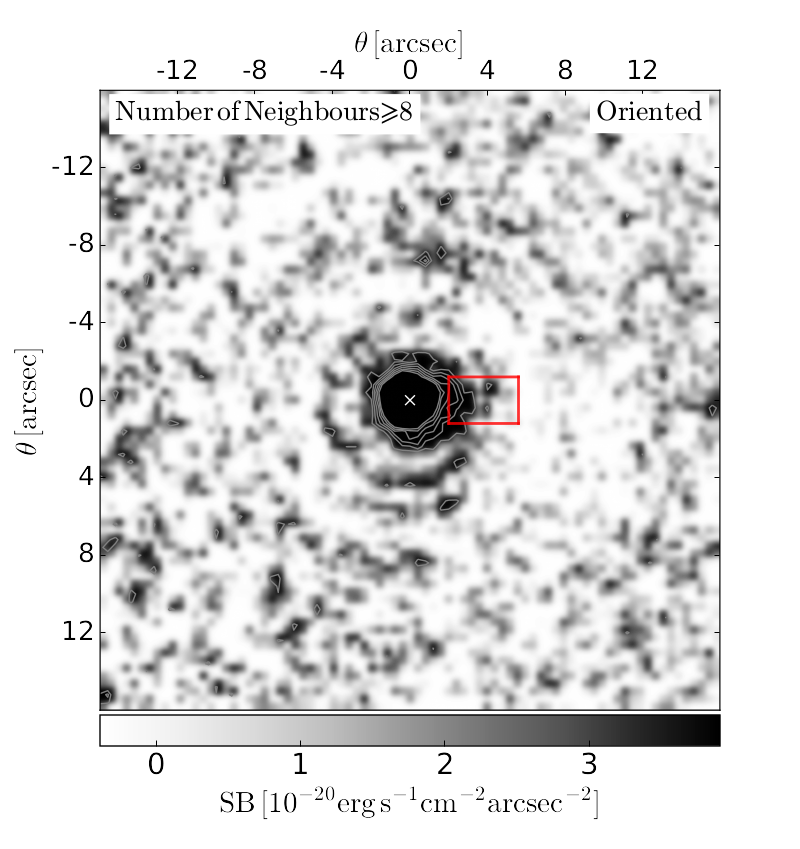
\includegraphics[height=10cm]{SG/stack-nmin8.png}
    \end{center}
  \end{minipage}

  \vspace{0.5cm}

  {\footnotesize \textit{[Gallego, Sofia G. et al. 2017, arXiv:1706.03785]}}
\end{section}